 

\subsection{Shape Refinement}\label{sec:refinement}
 
Though not perfect, the initial 3D shape provides a good starting point for generating the final carton model. 
To further refine the 3D shape, the 3D coordinates of all the vertexes are then refined based on a set of shape constraints, such as vertex merging, panel pasting, and so on.
In this step, the coordinates of vertexes are chosen as our objective instead of angles on folding edges, mainly because that the geometric constraints in 3D shapes can be more simply and intuitively represented by 3D vertex coordinates. 
 
A suggestive interface is provided to users to efficiently explore better carton shapes, as described later in Sec.~\ref{sec:interaction}. 
%
Once the user selects a suggested shape refinement operation, we optimize the 3D shape based on a series of geometric constraints. 
Given the current mesh with vertex positions that are defined as $\{\vo_i\}^{N}_{i=1}$, a new mesh with the same topology but new vertex positions $\{\vn_i\}^{N}_{i=1}$ is computed according to the specified shape constraints.
%
The geometric constraints can be classified into two groups, shape rigidity constraints and shape modification constraints.
% 
First, to keep the rigidity of each panel, the shape rigidity constraints, including panel rigidity and coplanarity, correspond to the similarity constraint and plane constraints described in \cite{Bouaziz:2012:SSD:2346796.2346802}. 
%
Second, once the vertexes or panels are confirmed to be merged to modify the rough shape, more modification constraints are added. 
%
Each constraint is defined accordingly.  
 

\paragraph{Panel rigidity.} 
Each panel maintains its shape during the folding process. This constraint is defined by keeping the distance between any pair of points $\mathbf{v}_{a}, \mathbf{v}_{b}$ on the panel the same.
\begin{equation}
||\mathbf{v}_{a} - \mathbf{v}_{b}||^2 - ||\hat{\mathbf{v}}_{a} - \hat{\mathbf{v}}_{b}||^2 = 0.
\label{equ:plane}
\end{equation}



\paragraph{Coplanarity.} For each panel $P_{k}$, the coplanarity constraint specifies that all vertexes in this panel should always lie on a plane. 
We compute the sorted eigenvectors $\mathbf{U} = [\mathbf{e}_1, \mathbf{e}_2, \mathbf{e}_3]$ of the $ 3 \times 3$ covariance matrix $\mathbf{C}^T\mathbf{C}$ where $\mathbf{C} = \{\mathbf{v}_{kj}\}_{j=1}^{N_k}$, $\mathbf{v}_{kj}$ is the $j^{th}$ vertex among $N_k$ vertexes in the panel. By removing the last column of $\mathbf{U}$, we implement the plane projection as \cite{Bouaziz:2012:SSD:2346796.2346802} described.
\\

If a set of shape modification operations, such as vertex merging and panel pasting, are selected, more constraints are added to optimize the vertex positions. 

\begin{figure}
	\centering
	\subfigure[Vertex Merging]{
		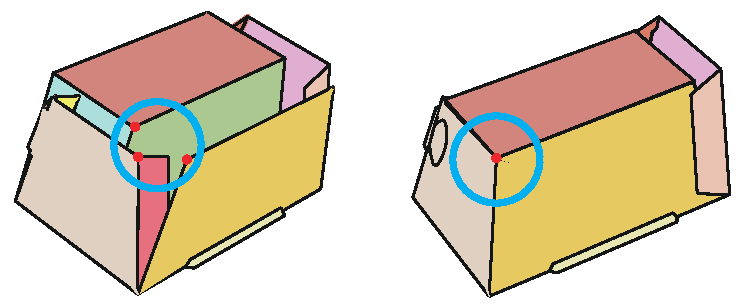
\includegraphics[width=0.45\columnwidth]{images/vertexmerging}
		\label{fig:vertexmergingBeforeAfter}
	}
	\hfill
	\subfigure[Panel Pasting]{
		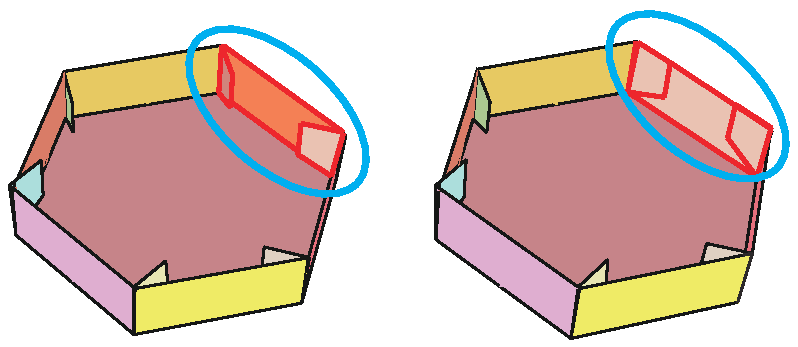
\includegraphics[width=0.45\columnwidth]{images/facemerging}
		\label{fig:facemergingBeforeAfter}
	}
	\caption{3D shape refinement based on merging vertexes (a), or pasting panels (b). The locations where the 3D shape changes are circled in blue.  }
	\label{fig:shaperefinement}
\end{figure}

\paragraph{Merging vertexes.} 
For any two vertexes, $\mathbf{v}_p$ and $\mathbf{v}_q$, that are selected to be merged as the same vertex, we have:
\begin{equation}
\mathbf{v}_p - \mathbf{v}_q = \mathbf{0}.
\label{equ:point}
\end{equation}

\paragraph{Panel pasting.} 
If two panels, $P_a$ and $P_b$, need to snap together, all the vertexes from these two panels should satisfy the same coplanarity constraint. 
 
Typically only a few shape modification operations are selected at each time; the above constraints form an under-constrained system to solve the new vertex coordinates. In order to find a feasible solution for the constrained problem, soft constraints are added to keep the original positions of the vertexes that are not relevant to the selected shape modification.

\paragraph{Irrelevant vertexes.} 
Vertexes that are not in the same panel as any merged or pasted vertexes should remain in their original locations.
We add these soft constraints by adding a small weight $w$, which is set to 0.001 in our experiments to the following equation:
\begin{equation}
w(\mathbf{v}_i - \mathbf{\hat{v}}_i) = \mathbf{0}.
\label{equ:irrelevant}
\end{equation}

Bouaziz et al.~\cite{Bouaziz:2012:SSD:2346796.2346802} proposed an efficient optimization method to combine all these shape constraints together. We directly use their C++ library, ShapeOp, to solve our shape optimization problem once a shape modification operation is performed.
Figure~\ref{fig:shaperefinement} shows two examples of shape refinement by merging three vertexes and pasting three panels, respectively. 
 
% 


%

